\chapter{Variability in network architecture and its relationship to reading}

\section{Motivation}

How variable is task-evoked functional connectivity, and is it indicative of greater efficiency? Is greater variability in network architecture a feature beneficial attribute -- or is it indicative of a less efficient organization?

In Study 1, we established that the degree of global modularity -- a key component of an efficient small-world architecture -- of an individual's connectome at rest is positively associated with reading skill. The exception to this was in the cingulo-operculuar and auditory networks, which had a negative correlation; that is, lower segregation of these areas was associated with better reading. In Study 2, we found that reading comprehension induced a more integrated network architecture as information was shared across RSNs. However, the relationship between reading skill and modularity persisted, even as connectomes were estimated during separate conditions. 

It thus appears that variability in network architecture across different tasks may not be indicative of high readers. Rather, these results would suggest that better readers have a common and tightly connected network ``backbone'' that is persistent throughout task reconfiguration. Given that reading is a skill that we know requires a very high degree of cross-RSN interaction, we might expect this to be true in a variety of other domains as well. In fact, we might expect that there would be a high degree of consistency between a number of different tasks: listening and reading, but also more basic attention and resting states. 

In this third study, we expand our task and analyses to encompass the auditory modality in order to address two questions:

\begin{itemize} 
	\item Do better readers have greater similarity between listening and reading network parcellations?
	\item To what extent does flexibility in network organization predictive of individual differences in cognitive measures?
\end{itemize} 

Below, we motivate these two aims individually.

\subsection{The connectome in language comprehension}


The most widely-held view is that reading and listening share the same core linguistic processes and differ primarily in the sensory processes that feed into supra-model linguistic systems \citep{Mattingly1971, Price2012}. One popular model, the \textit{Simple View of Reading} states that reading comprehension is the product of listening comprehension and decoding skills \citep{Gough1986}. This view has received support from large behavioral studies \citep{Kirby2008} and neuroimaging investigations: many of the literacy-related changesare linked to visual or phonological systems, areas not directly related to semantic or comprehension processes \citep{Schlaggar2007, Dehaene2015}. These findings support a model in which inputs from auditory or visual domains are fed up into higher-order association areas that sequence, encode articulatory plans, and extract semantic information \citep{Price2012}. These processes localize onto the similar areas regardless of language and writing system \citep{Rueckl2016}, and may even extend to inputs from somatosensory domains \citep{Xu2005, Sood2016}. This supra-modal language core is largely left-lateralized and centers on the inferior frontal gyrus, anterior and posterior middle temporal gyrus and the angular gyrus. Neuroanatomical models of language, shown in Fig. \ref{ch3-price-language-models}, illustrate that language is distributed throughout much of the brain. 

There exists a common core architecture for reading and listening. The models presented here contend that reading and listening share the same core processes, with the major differences being in the sensory processing functions.

\begin{figure}[t]
	\centering
	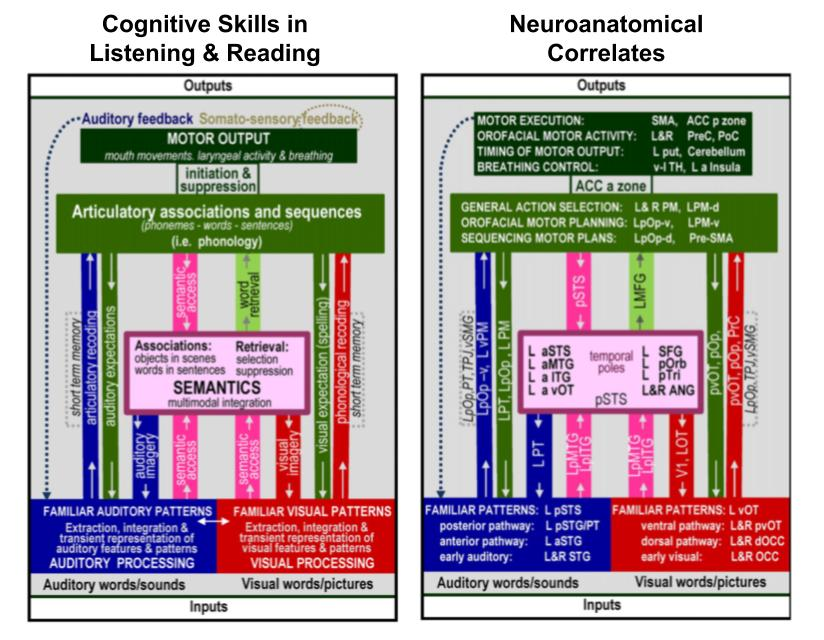
\includegraphics[height=3in]{ch4-price-language-models}
    \caption[Common core architecture for reading and listening.]{There exists a common core architecture for reading and listening. The models presented here contend that reading and listening share the same core processes, with the major differences being in the sensory processing functions. Figure adapted from \citep{Price2012}.}
	\label{fig:ch4-price-language-models}
\end{figure}

Brain activation studies have noted that reading is marked by greater intensity and extent of activation in supramodal language processing areas than listening, especially in developing readers \citep{Berl2010}. 

Most current cognitive models suggest that language comprehension requires the construction of a mental representation includes textual information and associated background knowledge, connected by some conscious and some unconscious executive processes \citep{Kendeou2014}. The parallel model shown in Fig. \ref{fig:ch4-price-language-models} is linear: it moves from sensation to action. During comprehension, however, the relationship between areas is dynamic and constantly being re-evaluated. The roles of attention and executive systems are likely to play an important role. Thus, while there may be a core set of systems for manipulating and extracting meaning from language, it is likely that differences in modality would modulate these processes. 

However, it may may not capture these differences: it could very well be the interactions of different functional systems that are changed, rather than the overall ``engagement'' of an individual brain area. Additionally, the fact that reading integrates in an additinoal modality could be a source of difference, especially in emerging readers. 

Despite the clear overlap between reading and listening, there is also evidence that the two skills are not directly equivalent. The pioneering researcher Alvin Liberman suggested that reading is parasitic on listening: it requires the majority of the listening machinery, as well as an awareness of the linguistic act \citep{Mattingly1972}. There is a subset of students who, despite adequate word decoding skills and vocabulary skills, struggle with reading comprehension\citep{Pimperton2010, Spencer2014}. From a neurobiological perspective, expected differences in primary visual (for reading) and primary auditory (for listening) represent the different input systems, with ventral occipito-temporal systems also activating \citep{Jobard2007}. However, differences in core language systems are also observed: additional activation in left posterior temporal and parietal areas in reading modality \citep{Constable2004}, as well increased bi-laterality especially in children \citep{Berl2011}. 

\subsection{Variability in connectomes}

The ``flexible hub'' theory asserts that a subset of regions in the brain are responsible for coordinating other brain systems in the accomplishment of internally-directed aims \citep{Cole2007}. Hubs provide a way in which the brain might maintain its overall modular architecture while still increasing communication between regions. While there are a number of cognitive systems that may perform hub-like functions, including the salience, dorsal attention, ventral attention, and cingulo-opercular networks, several researchers have targeted the front-parietal network as a particularly important set of areas likely to perform hub-like functions \citep{Cole2013, Niendam2012}. One reason is that it encompasses the lateral prefrontal cortex, which has been seen to exert top-down control over other brain areas and which is often active in novel or difficult tasks \citep{Duncan2010}. Global functional connectivity in the fronto-parietal network has also been shown to predict individual differences in cognitive skills and intelligence \citep{Cole2012}. Taken together, there is significant evidence for the importance of hub regions in supporting flexible cognition, and the fronto-parietal network may be particularly important. 

% Task-based neuroimaging provides us with a rich description of the functions of frontoparietal network. The frontoparietal network is an assembly of brain regions encompassing the lateral frontal and parietal cortices along with insular, anterior/mid cingulate, and inferior temporal areas that have been broadly implicated in a variety of higher-level cognitive tasks \citep{Fedorenko2013}. Some have described the frontoparietal network as supporting active and adaptive online control, initiating and adjusting goal-directed mental systems \citep{Dosenbach2007}, while others have proposed a more general superordinate role in directing cognition \citep{Niendam2012}. The most obvious relationship of the frontoparietal network to language is its proximity to Broca’s area, known for its critical role in language articulation. Rather than thinking of this area (traditionally, Brodmann areas 44 and 45) as exclusively or primarily language-related, it has been argued that Broca’s area supports hierarchical executive processing, such as the segmentation (``chunking'') of auditory language and the flexible combination of words \citep{Koechlin2006}. Thus, while Broca's area plays a role in the unification of representations, prefrontal cortex (and the larger frontoparietal network) may play a higher-level control and initiating role in language and other processes \citep{Hagoort2005}. 


We have seen previously that global and regional network architecture changes during task activation, but that its overall preservation of a modular architecture is important for skilled reading. A subsequent question is, what attributes of the network architecture enable flexibile reorganization while also preserving modularity? Strong candidates for this role are variability in the hub regions, but these should also show flexibility across a number of tasks -- not just listening and reading, but other cognitive tasks as well. 

\subsection{Study aims}

The aims of the present study were to determine to what extent ``flexibility'' across different tasks is predictive of differences. On the one hand, we have evidence that modularity within the global network, in any condition, is predictive of reading skill. On the other hand, we know that different skills rely on different brain areas and require radically different organizations. We test two hypotheses in this study. First, that \textit{similarity} between listening and reading network architecture will correspond to higher reading skill Second, that \textit{dissimilarity} among hub-like areas will correspond to higher reading skill, and that this dissimilarity will be present in hub-like areas. 

\section{Methods}

\subsection{Participants}

Participants were drawn from the same cohort of subjects included in Studies 1 and 2, and identical inclusion criteria for both demographic and scan motion were applied. However, additional measures related to the performance of the task were levied as described below. A total of 42 unique subjects and 142 scan sessions were included in the analysis. The demographics for these subjects are described in Table \ref{table:ch4-participants}.

\begin{table}[t]
	\renewcommand{\tabcolsep}{0.09cm}
	\centering
	\begin{tabular}{lc}
\toprule
Measure &               Value \\
\midrule
Subjects                        &              42 \\
Mean age                        &    10.51 (0.33) \\
Sex                             &      21 M, 23 F \\
WASI Full-Scale IQ, Vocabulary  &    52.91 (9.38) \\
Test of Word Reading Efficiency &  104.66 (18.07) \\
\bottomrule
\end{tabular}
	\caption[Participant demographics for Study 3.]{Participant demographics for Study 3. Participants were a subset of those examined in Study 2, who had completed a listening comprehension task with sufficiently high quality.}
	\label{table:ch4-participants}
\end{table}

\subsection{Functional MRI acquisition and processing}

The task design for this study is described in detail in Chapter 3. Briefly, subjects were presented up to four separate runs of a language comprehension task. The task included two passage blocks (``Reading'' or ``Listening''), two sensory baseline blocks (``Attention'') and a trailing resting-state block ("Rest"). The four scan runs were crossed on two conditions: the modality of presentation (auditory or visual) and the genre of the passage (narrative or expository). 

A scan session was excluded based on the following parameters: the number of high-motion volumes exceeding 20 percent, mean frame-wise displacement greater than 0.4, or poor task performance ($D^\prime < 2$). To control for the effects of genre, we matched all scans that met inclusion criteria with their opposing-modality counterpart, so that each subject had either 2 scans (same genre in listening and reading) or 4 scans (both genres in listening and reading). In total, 42 children (142 scans) met inclusion criteria.

Functional MRI acquisition and preprocessing procedures were equivalent to those described for Study 2. See the \textit{Methods} section of Chapter 3 for a detailed description of these processes and their parameters.

\subsection{Activation and network analyses}

Our analysis was broken into two parts: first, comparing the similarities and differences in network organization for listening and reading, then across all available tasks. 

For the modality comparisons, we used a fixed-effects subject-level model to estimate the shared activation for ``Listening and Reading'' and their differences ``Listening vs. Reading''. We then used FSL's \textit{randomise} utility to estimate the main effects of modality across all subjects in our sample (5000 permutations, threshold-free cluster enhancement, $p < 0.05$).  We also investigated these effects in ``connectome space'' by extracting the values at each of the 264 nodes used for connectivity analysis, then comparing the activity profile of each RSN during reading and listening.

\subsection{Network similarity estimation}

Global modularity provides one estimate of network similarity, by comparing each network to a standard parcellation: two networks with high modularity using a given parcellation indicates that they share a high degree of commonality, especially within-RSNs. However, this has the drawback of being biased towards the provided RSN parcellation: two networks could receive the same low modularity scores, even if they deviated in totally different ways (i.e. were not similar). 

\begin{figure}[t]
	\centering
	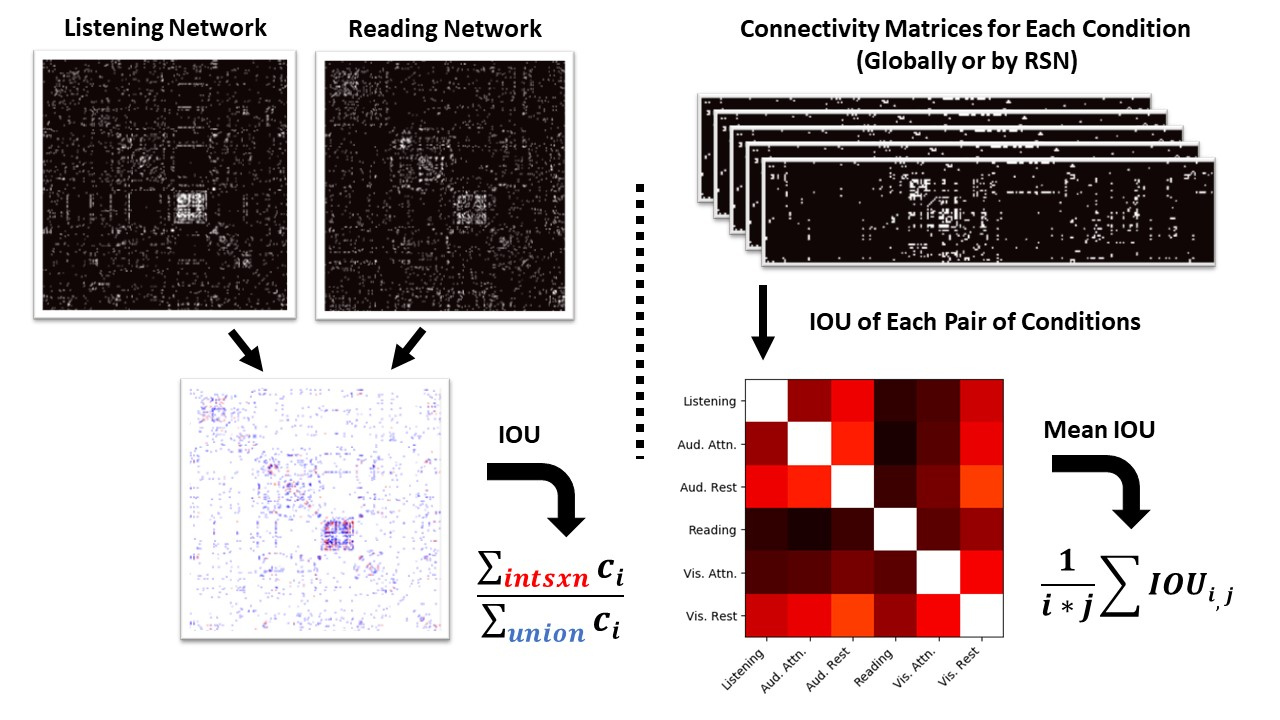
\includegraphics[height=3in]{ch4-network-similarity-methods}
    \caption[Method for comparing connectivity arrays.]{The network similarity measure provides a way of comparing connectivity arrays without reference to a pre-defined network parcellations.}
	\label{fig:ch4-network-similarity-methods}
\end{figure}

A less biased similarity metric would be based off of the \textit{intersection} of the two metrics, or the number of shared connections. This is particularly appropriate in our case, where each connectivity array has been thresholded to keep an identical number of connections. In this case, all possible network comparisons will have the same number of possible shared connections, so the number of actual shared connections is a stable metric for comparing between individuals or conditions. (For example, when thresholding for the top 5 percent of connections of a $264 * 264$ array, there is an upper limit of 3484 shared connections between two arrays.) 

We first compared the mean similarities of network arrays across individuals within the two linguistic conditions: listening to listening and reading to reading. We summarized the distributions of these similarites, with the expectation that there would be the most variability within the reading condition, since listening is more ``natural''. Next, we tested whether the similarity between an individual's reading and listening network arrays was related to reading skill. Finally, we RSN-level patterns of similarity and difference between reading and listening, to identify both a common ``backbone'' and a flexible ``periphery''. 

Next, we broadened the scope of analysis to include comparisons between all task conditions: rest, attention, and passage (across both conditions). For each subject, we created a similarity matrix describing the shared connections between each of these conditions. Then, we extracted the mean and standard devation of the shared connections. The question we were interested in was whether, within-subject, individuals who had fewer changes in state were also better cognitive performers. We then sought to determine whether changes within a single RSN (e.g. the fronto-parietal network) were the key drivers of this. 

\section{Results}

\subsection{Behavioral results}

Attention and comprehension measures were not related to modality of stimulus presentation. There was a trend towards difference in median FDRMS between scan modalities (paired t-test, $t = 1.94$, $p = 0.059$), so we also replicated analyses with a stricter motion threshold (no more than 10 percent outliers in a scan run). The main results from analysis of this 35 subject (116 scan runs) cohort were broadly consistent.

\subsection{Activation results}

As expected, reading and listening shared a common core of language-related activations. These included the bilateral middle temporal and inferior frontal gyri, as well as the  anterior temporal poles. The differences related to modality fell into three categories: sensory processing areas, including the insula, superior temporal gyrus, and secondary visual processing areas; and hetero-modal association areas, most notably the inferior frontal gyrus and angular gyrus; and somato-motor regions, including the premotor cortex and lateral geniculate nucleus of the thalamus (Fig. \ref{fig:ch4-modality-comparison-attn}). Areas showing greater activation in listening were focused on primary auditory cortex and the dorsal attention network.

\begin{figure}[t!]
	\centering
	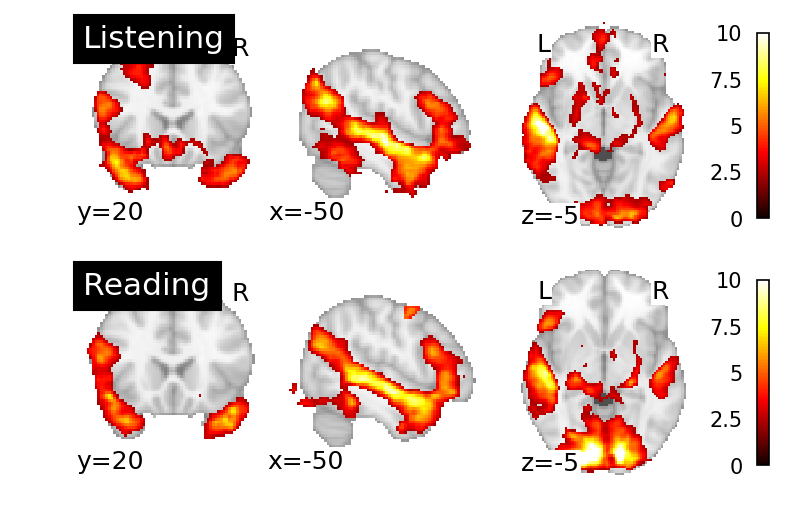
\includegraphics[height=3in]{ch4-modality-comparison-attn}
	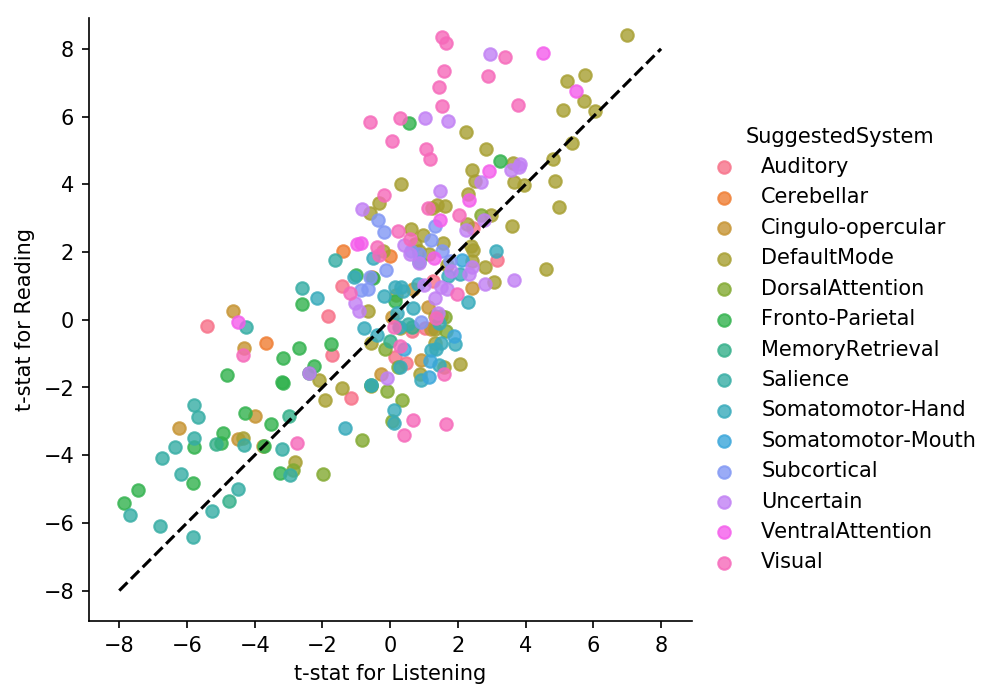
\includegraphics[height=3in]{ch4-listening-reading-connectome-activation-attn}
    \caption[Large overlap between listening and reading activation.]{There was a large overlap in activations between the listening and reading comprehension tasks. Activation spanned a bilateral set of regions, especially around middle temporal, inferior frontal gyri. Activations shown for $p < 0.05$, threshold-free cluster enhancement (5000 permutations).}
	\label{fig:ch4-modality-comparison-attn}
\end{figure}

This result is more easily visualized when viewing it in terms of the 264 nodes of the connectome. There was a very high correlation coefficient between activation during reading and listening ($p < 0.001$), reflecting the high degree of shared activity patterns between listening and reading. In general, areas that are active during listening are also active during reading, with the main differences falling into the sensory networks. 

\subsection{Network results}

In terms of graph theory measures, we found a significant decrease in modularity and a significant increase in participation coefficient in reading compared to listening (top of Figure  \ref{fig:ch4-modality-graph-theory}). This reflects that greater demands of reading, especially visually. 
\begin{figure}[t!]
	\centering
	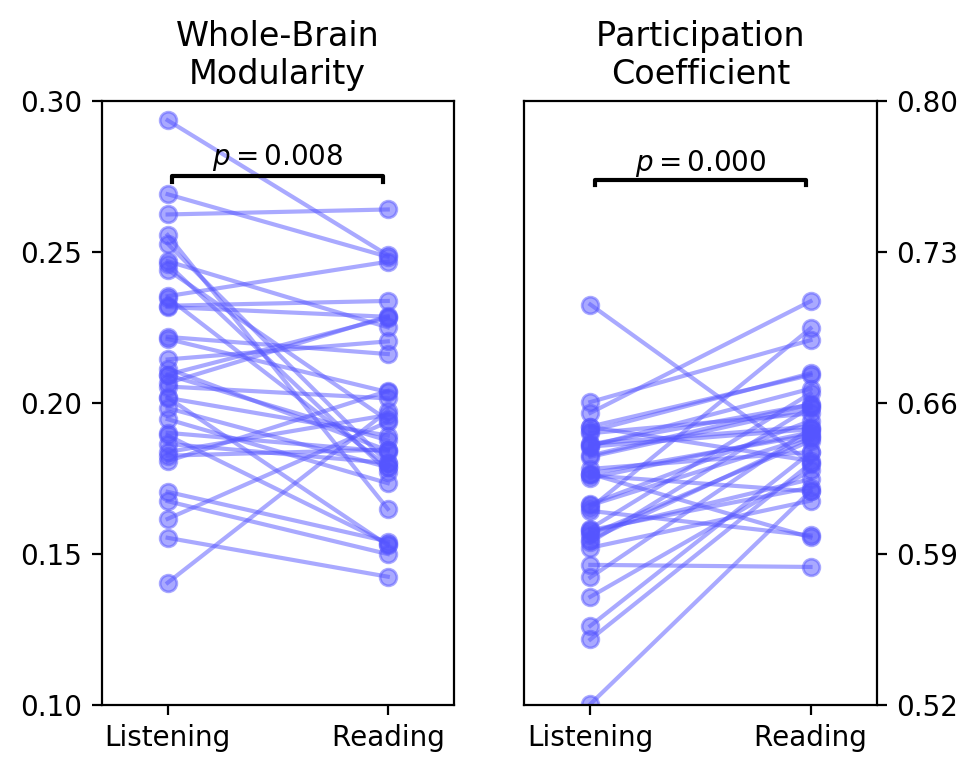
\includegraphics[height=3in]{ch4-modality-graph-theory}
	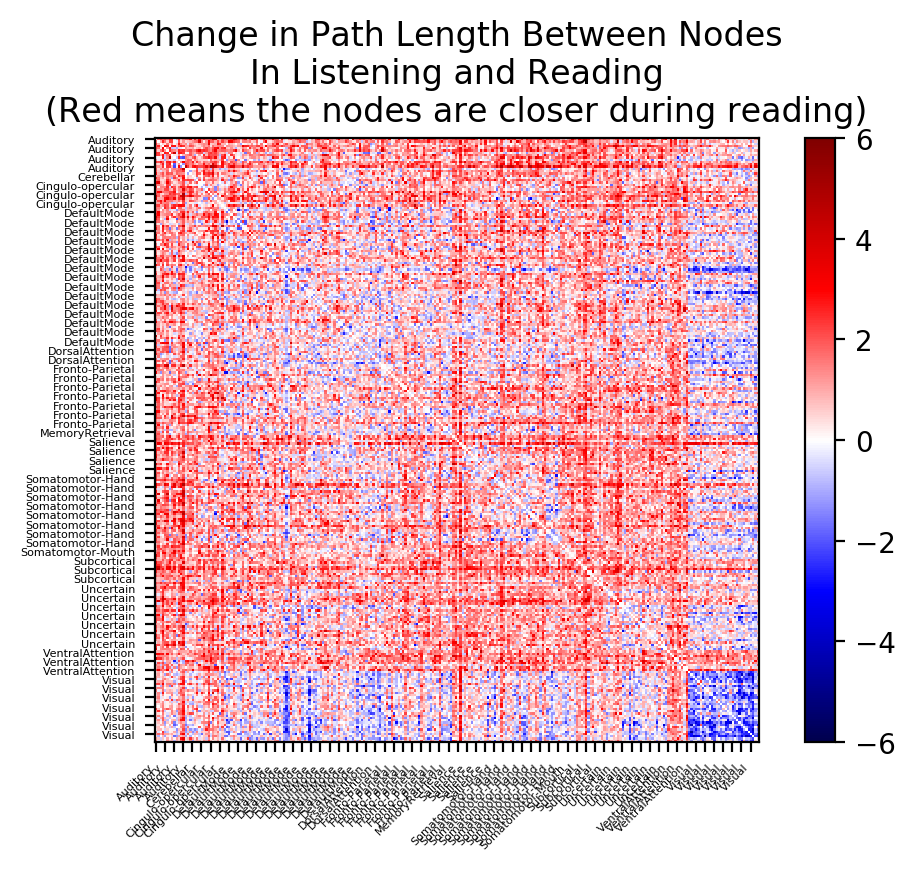
\includegraphics[height=3in]{ch4-modality-node-distance}
    \caption[Reading induces a more integrated network architecture than listening.]{Reading induces a more integrated network architecture than listening. In terms of modularity and participation coefficient, there is greater integration during reading than listening. }
	\label{fig:ch4-modality-graph-theory}
\end{figure}

Investigating the differences in path length between the two modalities provides a stronger sense of key drivers of this increased integration. The bottom panel of Figure \ref{fig:ch4-modality-graph-theory} displays the node-level connections of nodes that get closer or further during the reorganization. For the modality contrast, one of the main takeaways is that there is greater access between auditory and other areas during reading. this runs counter to our hypothesis that there would be less access to these areas. Visual areas, on the other hand, show less internal connectivity, reflecting the de-clustering of these areas during reading. 

\subsection{Network similarity results}

We next investigated whether different individuals evoked language-architectures that were similar to each other. For each pair of participants and modality of presentation, we totalled the number of shared connections between the two thresholded connectomes. We found that subject connectomes were much more similar when comparing ``listening'' connectomes than when comparing ``reading'' connectomes ($t = ...$, $p = ...$). Additionally, we found that subjects with the highest mean similarity overall were also more similar to other high-similarity subjects, suggesting that they are each approximating a common architecture during the comprehension process (see top panel of Figure \ref{ch4-modality-network-similarity}).

% Remove the l-t-r matrix and histogram... move to scatterplot below
\begin{figure}[t]
	\centering
	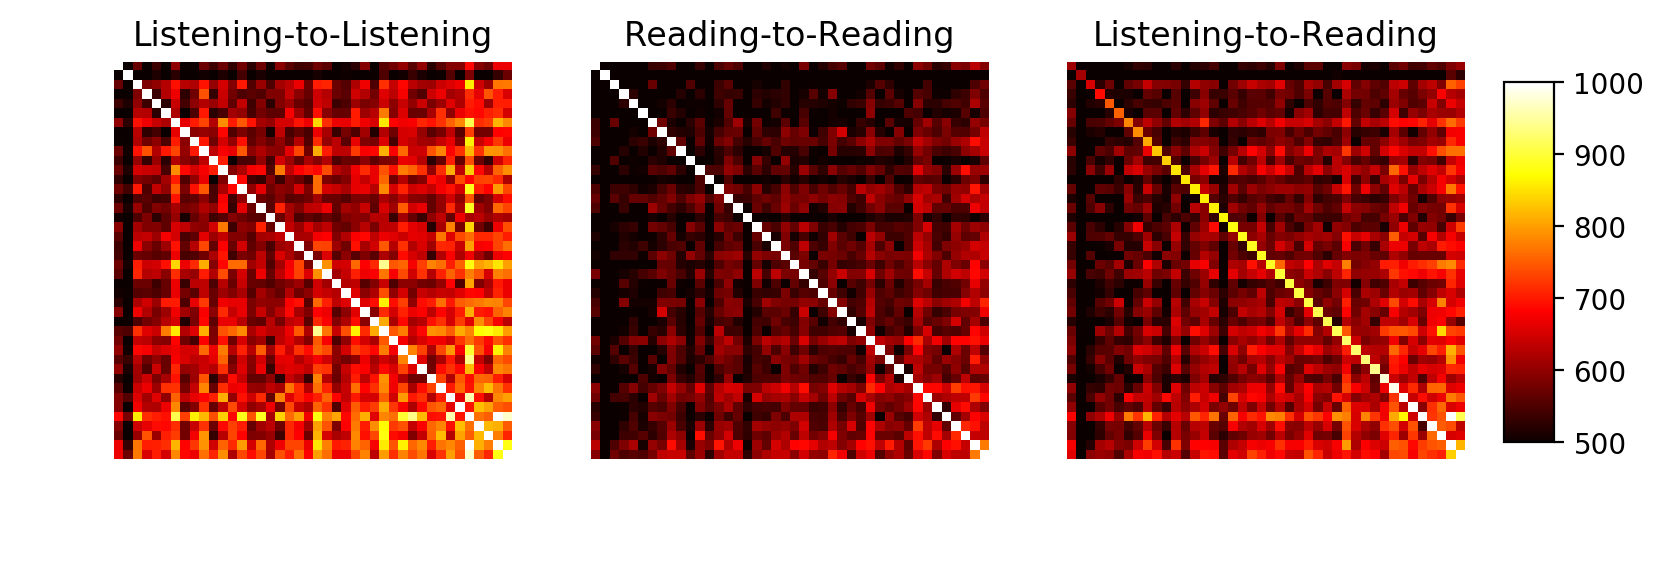
\includegraphics[width=5.5in]{ch4-modality-network-similarity}
	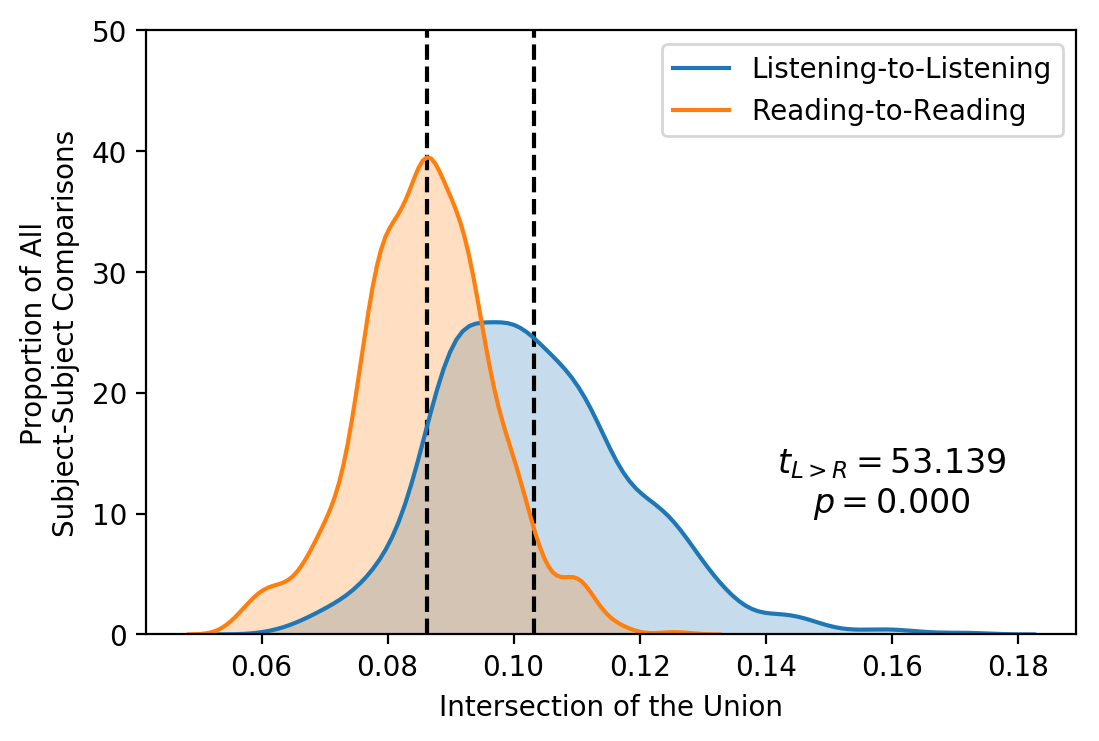
\includegraphics[width=5in]{ch4-similarity-condition-histogram}
    \caption[Network similarity across subjects in listening and reading.] {Network similarity across subjects in listening and reading. Across all participants, there is more shared network similarity in listening than there is in reading.}
	\label{fig:ch4-modality-network-similarity}
\end{figure}

As readers become more experienced, the expectation is that the task-evoked network architecture for reading would become more similar to that of the ``natural'' listening comprehension system. To test this, we compared each subject's listening network with their reading network then correlated this measure with TOWRE scores. We found that, indeed, better readers had a higher degree of similarity between the listening and reading networks ($r = 0...$, $p = ...$). Furthermore, we found that better readers shared more of their network structure with all readers, in every modality (two-sample $t$-test between top half and bottom half...). 

\begin{figure}[t]
	\centering
	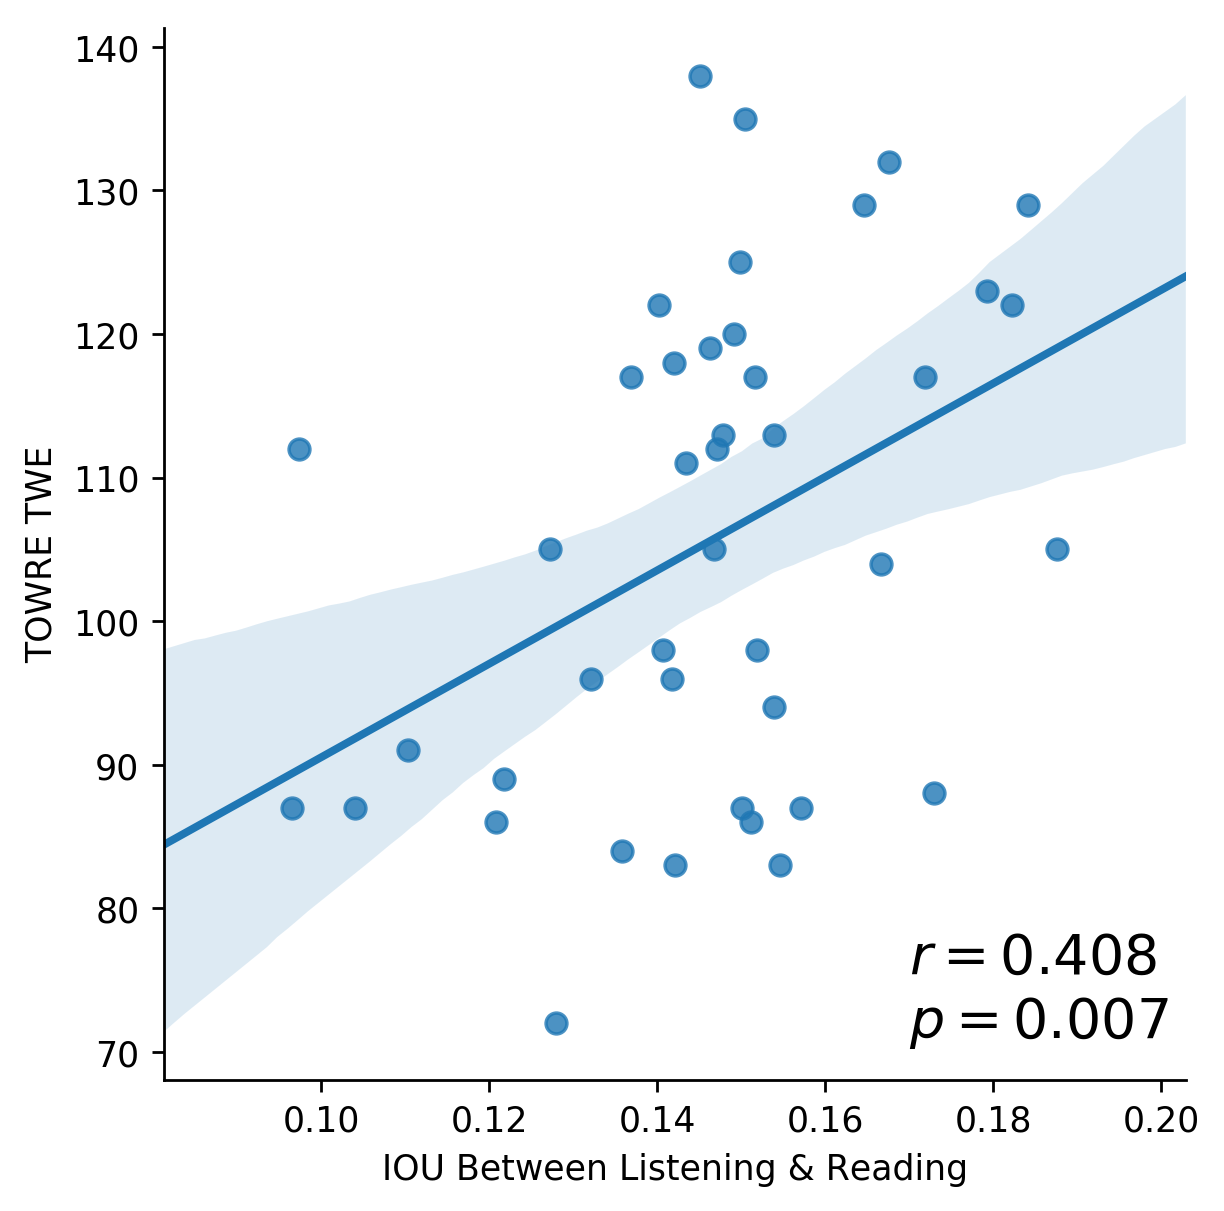
\includegraphics[height=3in]{ch4-modality-similarity-to-reading}
    \caption[Network similarity between listening and reading predicts word efficiency.]{Network similarity between listening and reading predicts word efficiency. We compared the listening parcellations to the reading parcellations for each pair of subjects.}
	\label{fig:ch4-modality-similarity-to-reading}
\end{figure}

Finally, we sought to determine whether there was greater variability across all tasks, and whether this was indicative of subject-level differences...
% Look at nodes that show increased participation coefficient across each different task. 
% Look at the fronto-parietal network, and determine whether DISSIMILARITY among the different parcellations is predictive of reading skill

% \begin{figure}[t]
% 	\centering
% 	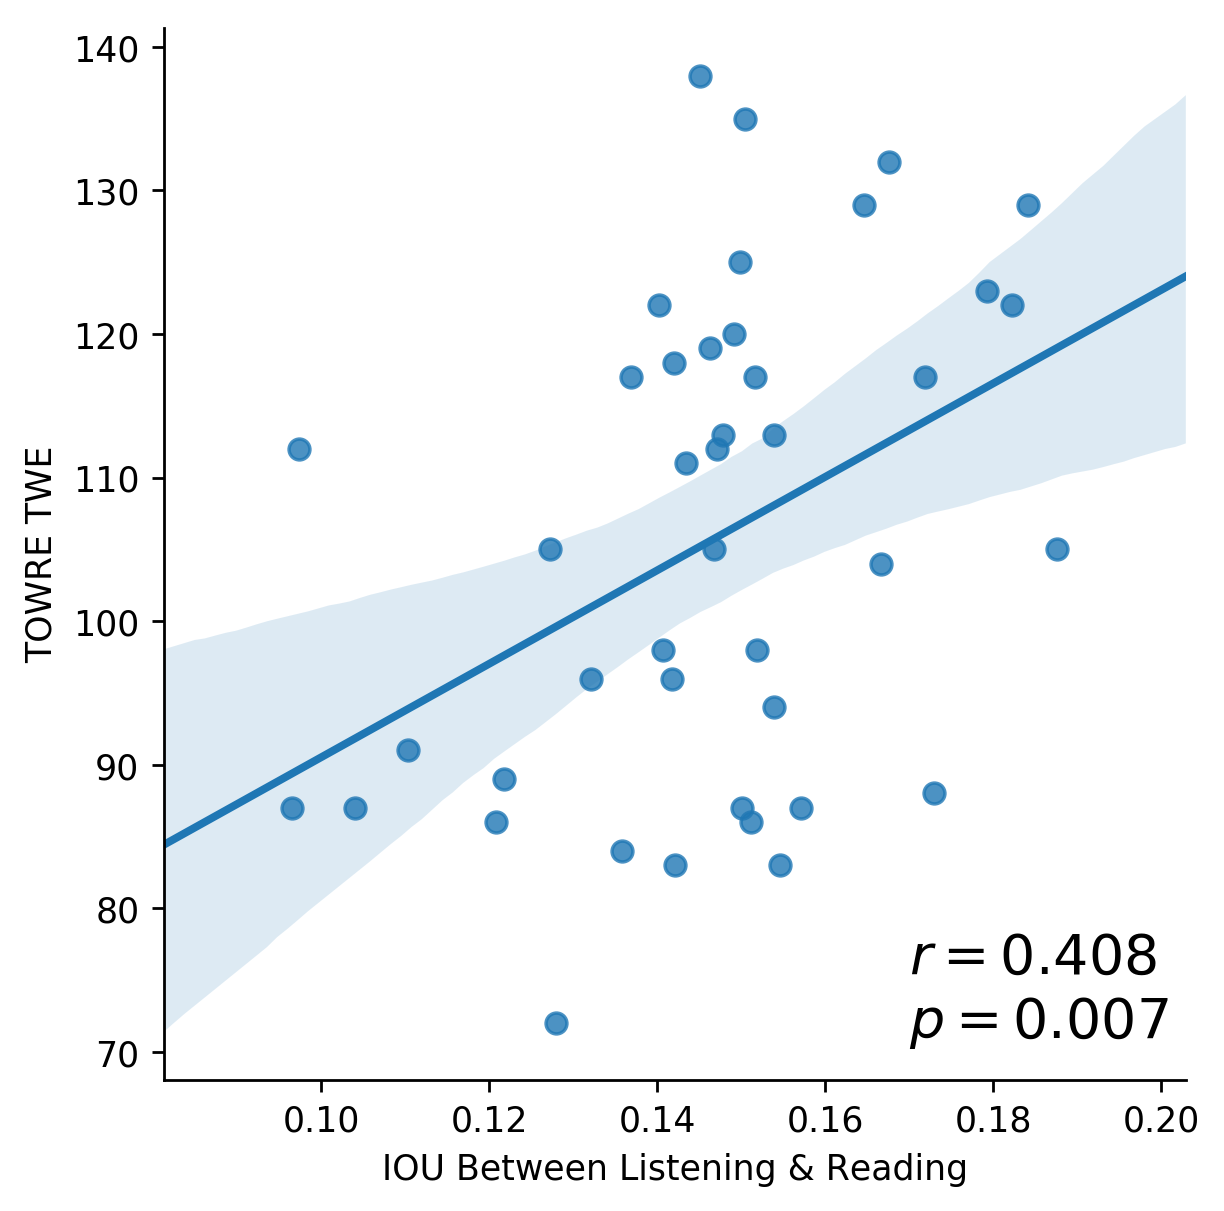
\includegraphics[height=3in]{ch4-modality-similarity-to-reading}
%     \caption[Network similarity between listening and reading predicts word efficiency.]{When projected into the node space, there was very strong correlation between activity in one and the other.}
% 	\label{fig:ch4-modality-similarity-to-reading}
% \end{figure}


\section{Discussion}

% Recap study rationale and results
This study investigates the differences between reading and listening in terms of their activation of individual areas or the distribution of activity across the brain. We employ closely matched texts, large sample size, longitudinal sampling, and behavioral covariates. Comprehending extended text requires more than just sensory and linguistic processes. It also requires executive processes such as attention, working memory and inference. Since comprehension is a "whole-brain" activity, we here look at the reorganization of resting-state networks - to see how attention, executive and sensory systems are interacting during reading.

% Significance of modality effects
The results make clear that differences in reading are not isolated solely to sensory systems, although the visual system is the major driver. We tested three hypotheses related to global reorganization, sensory system changes, and interactions between executive and attention systems and sensory systems. These modality-specific influences on behavior and brain activity may arise from a few different sources: subject, linguistic and innate differences. For example, there are also differences in what is encoded in speech and text. The reading sciences pioneer Alvin Liberman noted that "speech is a complex code, while reading is a simple cipher" \cite{Mattingly1971}. Speech contains overt clues about the speaker, such as tone and prosody, and these can convey additional non-linguistic meaning for the listener. Reading, on the other hand, might be considered a more purely linguistic act, especially with computer-printed text. Reading may thus allow more room for self-generated situation models and more independent direction of thought. Furthermore, modality-specific aspects of the stimulus may influence the overall comprehension process; reading requires a level of spatial awareness -where one is at on a page, what happened in preceding paragraphs – and allows for the re-treading of information. Listening, meanwhile, requires the extraction of input from competing noises and sometimes the tracking of changing volume. 

% Significance of graph theory results - greater integration globally driven by visual ``de-clustering''
People speak differently than they write. Reading often relies on more complicated syntax, and even for skilled readers, longer words and sentences can strain executive systems more than they might if being spoken to. Although these properties are often controlled for in scientific studies, they represent a major difference between “natural” reading and listening. Because of these differences, reading may place a greater load on executive function skills. Executive functions such as working memory and planning and organizing may be particularly important for reading \citep{Cain2006}.  

% Significance of similarity results between modality
The last set of differences is particularly interesting because knowing how the differences in reading interact with these modality differences. Reading is a learned skill with may component processes. It requires thousands of hours of experience to master and entails a reorganization of cortical resources. Environmental and biological factors thus exert a greater influence on an individual’s reading proficiency than they might on more intrinsic processes such as speech comprehension. This is particularly dramatic in individuals with dyslexia, who have persistent difficulty with reading. Children with dyslexia exhibit less activation in reading-related areas compared to typically developing children \citep{Pugh2000}, but greater activation in right hemisphere homologues, suggesting that lateralization and activation of the reading circuit are associated with better reading. Development period also has an effect, with children exhibiting less activation in frontal areas but more in posterior areas, possibly reflecting a shift in “resource load” from uni-modal to supramodal areas \citep{Berl2011}. This shift may not be necessary in listening, or occur much earlier. Thus, with increasing expertise and development, there may be a “shift” from relying on fusiform processing areas. towards using multi-modal areas more like speech \citep{Monzalvo2013}. 

% Significance of hub / vairability measures in fronto-parietal network

% Attention networks
% While we found an expansion of the left frontoparietal RSN to regions of the ventral attention RSN in good readers, we did not find an association between variation in the ventral attention RSN itself and individual differences in reading ability. The ventral attention network detects salient or unexpected stimuli in the environment \citep{Vossel2014}. In this way the ventral attention network can act as a ‘circuit breaker’ for the dorsal system to help reorient attention \citep{Corbetta2002}. It may thus help orient individuals to new information from the visual environment (i.e. text) and, by coupling stimulus-driven attentional areas with the frontoparietal network, it may help construct updated mental representations of linguistic material. The leftward aspects of the ventral attention network underlie crucial reading-related areas, including occipito-temporal cortex, which performs orthographic processing, and temporo-parietal cortex, important for semantic binding \citep{Taylor2013}. The absence of reading-related variance associated with the entire bilateral RSN may reflect the diversity of functions that these areas serve in basic visual and auditory processing, as well as language and reading. 


% Conclusions... development